\chapter{Réalisation}

Ce chapitre présente la réalisation concrète de Smart Farm AI v3.0.
Nous décrivons d'abord l'environnement de travail — matériel, logiciel et
langages de programmation — puis les interfaces des neuf modules fonctionnels
de la plateforme, et enfin les résultats des tests et de la validation terrain
sur 7 fermes pilotes tunisiennes.

% ── 4.1 Introduction ─────────────────────────────────────────
\section{Introduction}

Ce chapitre clôt le mémoire en présentant la réalisation industrielle de
Smart Farm AI v3.0. Il couvre l'environnement de développement matériel et
logiciel, les langages et outils retenus, les interfaces réalisées pour
chacun des modules fonctionnels (Vision IA, Apiculture, Aviculture ERP,
Cartographie GIS, Agent Darija, Télémétrie IoT, PWA Worker), ainsi que les
résultats des tests de validation et de la campagne terrain sur
7 fermes pilotes tunisiennes (décembre 2025 -- avril 2026).

% ── 4.2 Environnement de travail ─────────────────────────────
\section{Environnement de travail}

L'environnement de développement de Smart Farm AI se compose de trois
dimensions complémentaires~: le matériel physique (station de développement
et nœuds IoT embarqués), les logiciels (IDE, conteneurisation, bases de données,
inférence LLM, MLOps) et les langages de programmation (Python, JavaScript,
SQL, YAML).

% ── 4.2.1 Environnement matériel ────────────────────────────
\subsection{Environnement matériel}

Pour réaliser notre solution, nous utilisons un ordinateur MSI. Les
caractéristiques de cet environnement matériel sont inscrites dans la
figure~\ref{fig:env_materiel}.

\begin{figure}[H]
\centering

\includegraphics[width=0.88\textwidth]{specification_pc.png}
\caption[Caractéristiques du matériel utilisé]{Les caractéristiques environnementales du matériau utilisé}
\label{fig:env_materiel}
\end{figure}

% ── 4.2.2 Environnement logiciel ────────────────────────────
\subsection{Environnement logiciel}

L'environnement logiciel de Smart Farm AI couvre l'ensemble du cycle de
développement~: édition du code, conteneurisation, persistance des données,
inférence IA locale et traçabilité MLOps.

\paragraph{Visual Studio Code.}
VS Code constitue l'unique IDE du projet, utilisé aussi bien pour le backend
Python (extensions Pylance, Black, Ruff pour le formatage) que pour le
frontend JavaScript (ESLint, Prettier). Le débogueur intégré permet
d'inspecter les requêtes FastAPI et les réponses du modèle YOLO en temps réel.

\begin{figure}[H]
\centering

\includegraphics[width=0.18\textwidth]{vscode.png}
\caption[Logo Visual Studio Code]{Logo Visual Studio Code — IDE principal du projet}
\label{fig:vscode_logo}
\end{figure}

\paragraph{Docker Desktop 25.0.3.}
Docker Compose orchestre 3 services actifs (+ Caddy optionnel HTTPS) :
\texttt{db} (PostgreSQL 16-alpine), \texttt{backend} (Python 3.11-slim + Uvicorn
2 workers) et \texttt{frontend} (Nginx 1.27-alpine servant le build React/Vite).
Les dépendances de démarrage sont gérées par \texttt{healthcheck}~:
\texttt{postgres} doit être \texttt{healthy} avant \texttt{backend} ;
\texttt{backend} avant \texttt{frontend}.


\begin{figure}[H]
\centering

\includegraphics[width=0.92\textwidth]{architecture_deploiement_docker.png}
\caption[Architecture de déploiement Docker]{Architecture de déploiement Docker --- 3 services actifs (Caddy optionnel),
ports réels, flux de communication}
\label{fig:deployment_arch}
\end{figure}

Le fichier \code{docker-compose.yml} orchestre les services principaux de la
plateforme en production. Le tableau~\ref{tab:docker} synthétise les images
utilisées et le rôle de chaque service.

\begin{table}[H]
\centering
\caption[Services Docker Compose]{Services Docker Compose en production (3 actifs + 1 optionnel)}
\label{tab:docker}
\small
\renewcommand{\arraystretch}{1.25}
\resizebox{\textwidth}{!}{%
\begin{tabular}{@{}p{2.4cm}p{3.8cm}p{8.2cm}@{}}
\toprule
\textbf{Service} & \textbf{Image} & \textbf{Rôle} \\
\midrule
\code{db} & \code{postgres:16-alpine} & Base de données principale avec volume persistant \code{postgres\_data}. \\
\code{backend} & Dockerfile (Python 3.11) & API FastAPI exécutée avec Uvicorn (2 workers), port 8000, intégration MQTT HiveMQ. \\
\code{frontend} & Dockerfile (nginx:alpine) & Build React/Vite servi par Nginx, port 80, proxy \code{/api/v1} vers le backend. \\
\code{caddy} & \code{caddy:2-alpine} & HTTPS automatique avec Let's Encrypt, service optionnel commenté par défaut. \\
\bottomrule
\end{tabular}%
}
\end{table}

\paragraph{PostgreSQL 16 + PostGIS.}
PostgreSQL 16-alpine héberge les 38 modèles SQLAlchemy du projet. L'extension
PostGIS permet d'exécuter des requêtes géospatiales telles que
\code{ST\_DWithin} avec le système de référence SRID~4326.

\begin{figure}[H]
\centering

\includegraphics[width=0.42\textwidth]{postgresql_postgis.png}
\caption[PostgreSQL 16 et PostGIS]{PostgreSQL 16 + PostGIS --- persistance et requêtes géospatiales}
\label{fig:postgresql_postgis}
\end{figure}

\paragraph{Ollama ($\geq$0.1.7).}
Ollama fournit un serveur d'inférence LLM local accessible sur
\code{localhost:11434}. Il héberge Labess-7B pour l'assistant Darija et
LLaVA-7B pour la vision multi-modale.

\begin{figure}[H]
\centering

\includegraphics[width=0.34\textwidth]{ollama.png}
\caption[Serveur local Ollama]{Ollama --- serveur local d'inférence LLM et vision multi-modale}
\label{fig:ollama}
\end{figure}

\paragraph{MLflow + DVC.}
MLflow assure la traçabilité des expériences d'entraînement, tandis que DVC
versionne les datasets et les modèles entraînés via des pipelines reproductibles.

\begin{figure}[H]
\centering

\includegraphics[width=0.46\textwidth]{mlflow_dvc.png}
\caption[Suivi MLflow et DVC]{MLflow + DVC --- suivi des expériences et versionnement des artefacts IA}
\label{fig:mlflow_dvc}
\end{figure}

\paragraph{GitHub.}
Le code source est versionné sur GitHub. Les pipelines CI/CD vérifient la
qualité du code et exécutent les contrôles Ruff, ESLint et pytest.

\begin{figure}[H]
\centering

\includegraphics[width=0.34\textwidth]{github.png}
\caption[Versionnement GitHub]{GitHub --- versionnement du code source et intégration continue}
\label{fig:github}
\end{figure}

% ── 4.2.3 Langages de programmation ─────────────────────────
\subsection{Langage de programmation}

Quatre langages ou formats sont utilisés dans le projet, couvrant le backend,
le frontend, la couche données et l'infrastructure : Python 3.11, JavaScript
/ React 18, Roboflow, SQL/PostgreSQL et YAML pour Docker Compose / DVC.

\paragraph{Python 3.11.}
Python 3.11 est utilisé pour développer le backend de la plateforme. Il permet
la création des endpoints FastAPI, l'intégration des modèles d'intelligence
artificielle, le traitement des images, la communication avec la base de données
et l'orchestration des services liés à l'analyse des données agricoles.

\begin{figure}[H]
\centering

\includegraphics[width=0.30\textwidth]{python.png}
\caption[Langage Python 3.11]{Python 3.11 --- langage principal du backend Smart Farm AI}
\label{fig:lang_python}
\end{figure}

\paragraph{JavaScript / React 18.}
JavaScript avec React 18 est utilisé pour la réalisation de l'interface web.
Il permet de créer des pages dynamiques, des composants réutilisables, des
visualisations interactives et une expérience utilisateur fluide pour les
profils Propriétaire et Ouvrier PWA.

\begin{figure}[H]
\centering

\includegraphics[width=0.30\textwidth]{react.png}
\caption[Frontend JavaScript / React 18]{JavaScript / React 18 --- développement de l'interface frontend}
\label{fig:lang_react}
\end{figure}

\paragraph{Roboflow.}
Roboflow est utilisé dans la préparation et la gestion des jeux de données de
vision par ordinateur. Il facilite l'annotation, l'organisation, l'augmentation
et l'export des datasets nécessaires à l'entraînement des modèles YOLO utilisés
par le module de détection intelligente.

\begin{figure}[H]
\centering

\includegraphics[width=0.36\textwidth]{roboflow.png}
\caption[Préparation des données Roboflow]{Roboflow --- préparation, annotation et export des données de vision IA}
\label{fig:lang_roboflow}
\end{figure}

\paragraph{SQL / PostgreSQL.}
SQL est utilisé pour manipuler les données persistantes de la plateforme.
PostgreSQL constitue la base de données principale, utilisée pour stocker les
fermes, les utilisateurs, les animaux, les mesures IoT, les diagnostics et les
données géospatiales exploitées par le module cartographique.

\begin{figure}[H]
\centering

\includegraphics[width=0.42\textwidth]{sql_postgresql.png}
\caption[Stockage SQL / PostgreSQL]{SQL / PostgreSQL --- stockage et interrogation des données de la plateforme}
\label{fig:lang_sql}
\end{figure}

\paragraph{YAML --- Docker Compose / DVC.}
YAML est utilisé pour décrire l'infrastructure et les pipelines du projet.
Il intervient notamment dans \code{docker-compose.yml} pour orchestrer les
services applicatifs et dans \code{dvc.yaml} pour structurer les étapes de
préparation, d'entraînement et d'évaluation des modèles.

\begin{figure}[H]
\centering

\includegraphics[width=0.48\textwidth]{docker_compose_dvc.jpg}
\caption[Configuration YAML]{YAML --- configuration de l'infrastructure Docker et des pipelines DVC}
\label{fig:lang_yaml}
\end{figure}

% ── 4.3 Réalisation ──────────────────────────────────────────
\section{Réalisation}

La réalisation de Smart Farm AI est organisée autour de deux espaces
fonctionnels complémentaires. Le premier espace est destiné au profil
\textbf{Admin / Owner}. Il regroupe les pages de gestion, de supervision et
d'aide à la décision utilisées par le propriétaire ou l'administrateur de la
ferme. Le deuxième espace correspond à l'application \textbf{Ouvrier PWA},
conçue pour un usage mobile sur le terrain avec un fonctionnement simple,
rapide et compatible avec le mode hors-ligne.

\begin{table}[H]
\centering
\caption{Pages principales de l'espace Admin / Owner}
\label{tab:pages_owner}
\small
\renewcommand{\arraystretch}{1.2}
\resizebox{\textwidth}{!}{%
\begin{tabular}{@{}p{4.3cm}p{10.5cm}@{}}
\toprule
\textbf{Page} & \textbf{Rôle fonctionnel} \\
\midrule
À propos du Projet & Présentation générale de la plateforme, de ses objectifs et de ses modules. \\
Tableau de Bord & Vue synthétique des indicateurs clés, alertes, statistiques et activités récentes. \\
Mes Fermes & Gestion des fermes, infrastructures, localisations et informations administratives. \\
Bétail \& Animaux & Suivi des animaux, espèces, états sanitaires, historiques et événements d'élevage. \\
Arbres \& Plantations & Gestion des cultures, plantations, parcelles et informations agronomiques. \\
Centre Cartographique & Visualisation GIS des fermes, points d'intérêt, vétérinaires et marchés. \\
Entrepôt & Suivi des stocks, ressources, équipements, intrants et mouvements d'inventaire. \\
Télémesure & Consultation des données IoT issues des capteurs et nœuds connectés. \\
Vidéosurveillance AI & Analyse vidéo et détection intelligente par modèles de vision artificielle. \\
Centre d'Alertes & Centralisation, priorisation et suivi des alertes critiques ou informatives. \\
Agri-Assistant (Derja) & Assistant conversationnel en dialecte tunisien pour l'accompagnement agricole. \\
Conseils AI & Recommandations intelligentes adaptées au contexte de la ferme et aux données collectées. \\
Rapports & Génération et consultation des rapports de suivi, performance et validation. \\
Paramètres & Configuration du compte, préférences, sécurité et paramètres de la plateforme. \\
\bottomrule
\end{tabular}%
}
\end{table}

\begin{table}[H]
\centering
\caption{Pages principales de l'application Ouvrier PWA}
\label{tab:pages_worker}
\small
\renewcommand{\arraystretch}{1.2}
\resizebox{\textwidth}{!}{%
\begin{tabular}{@{}p{4.3cm}p{10.5cm}@{}}
\toprule
\textbf{Page} & \textbf{Rôle fonctionnel} \\
\midrule
Accueil & Point d'entrée mobile présentant le résumé des tâches, l'état de synchronisation et les informations utiles. \\
Tâches & Liste des tâches assignées à l'ouvrier avec priorité, statut et validation terrain. \\
Scanner & Capture ou téléversement d'images pour lancer un diagnostic assisté par IA. \\
Signaler & Formulaire rapide pour remonter un incident, une observation ou une anomalie depuis le terrain. \\
Sync & Gestion de la synchronisation hors-ligne / en-ligne des actions enregistrées localement. \\
\bottomrule
\end{tabular}%
}
\end{table}

La plateforme propose deux flux d'authentification distincts. Le \textbf{Propriétaire}
se connecte via un formulaire email/mot de passe qui génère un token JWT HS256,
tandis que l'\textbf{Ouvrier PWA} valide son accès via PIN et OTP WhatsApp.

\begin{figure}[H]
\centering
\begin{subfigure}[b]{0.48\textwidth}
  \centering
  
\includegraphics[width=\linewidth]{screenshots/s_login_owner.jpg}
  \caption{Connexion Propriétaire --- authentification email/mot de passe et JWT HS256}
  \label{fig:screen_login_owner}
\end{subfigure}
\hfill
\begin{subfigure}[b]{0.48\textwidth}
  \centering
  
\includegraphics[width=\linewidth]{screenshots/s_login_worker.png}
  \caption{Connexion Ouvrier PWA --- validation PIN et OTP WhatsApp}
  \label{fig:screen_login_worker}
\end{subfigure}
\caption[Page d'authentification]{Page d'authentification --- connexion Propriétaire (JWT HS256) et Ouvrier PWA (OTP WhatsApp).}
\label{fig:screen_login}
\end{figure}

La sous-section suivante présente les captures réelles les plus représentatives
des deux espaces applicatifs : interface Propriétaire et application mobile
Ouvrier PWA.

% ── 4.3.1 Captures d'écran réelles de l'application ─────────────────────────
\subsection{Captures d'écran réelles de l'application}

Les captures d'écran suivantes illustrent l'interface réelle de Smart Farm
AI~v3.0 en cours d'exécution. Elles couvrent les modules principaux du tableau
de bord propriétaire (SPA React~18/Vite~5) et les écrans principaux de
l'application mobile Worker PWA (Android, mode hors-ligne). Les images sont
organisées selon les deux profils d'accès de la plateforme.

\subsubsection*{Interface Propriétaire}

\begin{figure}[H]
\centering

\includegraphics[width=0.88\linewidth]{screenshots/s01_landing.jpeg}
\caption[Page d'accueil de la plateforme]{Page d'accueil (Landing Page) --- point d'entrée unique avec accès distinct Propriétaire (JWT HS256) et Ouvrier PWA (WhatsApp OTP).}
\label{fig:s01_landing}
\end{figure}

La page d'accueil constitue le point d'entrée unique de la plateforme. Elle
présente l'identité visuelle de Smart Farm AI~v3.0 et propose deux boutons
d'accès distincts~: l'interface propriétaire et l'application mobile ouvrière.

\begin{figure}[H]
\centering

\includegraphics[width=\linewidth]{screenshots/s02_dashboard.png}
\caption[Tableau de bord principal]{Tableau de bord principal (Owner) --- KPIs temps réel, jauges IoT ESP32, carte GIS et alerte de détection de fumée d'incendie par YOLOv11.}
\label{fig:s02_dashboard}
\end{figure}

Le tableau de bord agrège en une vue unique les indicateurs critiques de
l'exploitation~: nombre d'animaux actifs, alertes non lues, température moyenne
IoT et production journalière. Les alertes sont diffusées par WebSocket et par
notification WhatsApp Business aux responsables de la ferme.

\begin{figure}[H]
\centering

\includegraphics[width=\linewidth]{screenshots/s03_livestock.png}
\caption[Module de gestion du bétail]{Module Gestion du Bétail --- inventaire par espèce avec fiches détaillées et score de santé individuel.}
\label{fig:s03_livestock}
\end{figure}

L'interface de gestion du bétail affiche les espèces suivies, le nombre de
têtes actives, le score de santé moyen et le statut d'alerte éventuel. Chaque
carte donne accès aux fiches individuelles, aux journaux de soins et aux
diagnostics IA associés.

\begin{figure}[H]
\centering

\includegraphics[width=\linewidth]{screenshots/s04_plants.png}
\caption[Module arbres et plantations]{Module Arbres et Plantations --- détection de maladies foliaires par YOLOv11 avec score de confiance et recommandation Darija automatique.}
\label{fig:s04_plants}
\end{figure}

Le module végétal permet l'analyse phytosanitaire par upload d'image ou capture
directe. Le modèle YOLOv11 affiche les boîtes englobantes colorées par classe,
le score de confiance et une recommandation de traitement générée par
l'assistant Darija.

\begin{figure}[H]
\centering

\includegraphics[width=\linewidth]{screenshots/s05_apiculture.png}
\caption[Module APICRAFT Apiculture]{Module APICRAFT Apiculture --- détection YOLO des abeilles et de la reine sur image de cadre de ruche.}
\label{fig:s05_apiculture}
\end{figure}

L'interface apicole APICRAFT intègre la détection visuelle des abeilles et de
la reine par modèle YOLO. Les résultats alimentent le suivi sanitaire de la
colonie et l'historique des diagnostics pour une analyse longitudinale.

\paragraph{Carte GIS.}
Le module GIS expose des endpoints GeoJSON REST pour les fermes, vétérinaires,
marchés, ruches et recherches de proximité, avec une double stratégie de calcul
de distance géographique : PostGIS en production et Haversine en fallback SQLite.
La formule Haversine utilisée est :
\begin{equation}
 d = 2R \cdot \arctan\left(\frac{\sqrt{a}}{\sqrt{1-a}}\right),\quad
 a = \sin^2\left(\frac{\Delta\phi}{2}\right) + \cos\phi_1\cos\phi_2\sin^2\left(\frac{\Delta\lambda}{2}\right).
\end{equation}

\begin{figure}[H]
\centering

\includegraphics[width=\linewidth]{screenshots/s05b_gis_map.png}
\caption[Carte SIG des fermes pilotes]{Carte GIS MapLibre GL / react-leaflet --- 7 fermes pilotes et 3 vétérinaires proches, recherche de proximité via Haversine (SQLite) ou \texttt{ST\_DWithin} (PostGIS)}
\label{fig:screen_gis}
\end{figure}


\begin{figure}[H]
\centering

\includegraphics[width=\linewidth]{screenshots/s06_warehouse.png}
\caption[Module entrepôt de la ferme]{Module Entrepôt de la Ferme --- gestion des stocks avec alertes de seuil minimal configurable et assistant IA.}
\label{fig:s06_warehouse}
\end{figure}

Le gestionnaire d'entrepôt organise les approvisionnements par catégories
(alimentation animale, médicaments, équipements, intrants et outils). Les seuils
minimaux déclenchent des alertes et facilitent le réapprovisionnement.

\begin{figure}[H]
\centering
\IfFileExists{figures/screenshots/s07_assistant.png}{%
  
\includegraphics[width=\linewidth]{screenshots/s07_assistant.png}%
}{%
  \placeholder{screenshots/s07\_assistant.png}%
}
\caption[Interface SovereignAssistant]{SovereignAssistant --- interface conversationnelle Darija avec historique des sessions, sources RAG ChromaDB et métriques qualité.}
\label{fig:s07_assistant}
\end{figure}

L'assistant souverain Darija offre une interface conversationnelle en dialecte
tunisien agricole. Il affiche l'historique des sessions, les sources RAG les
plus pertinentes et les métriques de qualité associées aux réponses générées.

\begin{figure}[H]
\centering

\includegraphics[width=\linewidth]{screenshots/s08_reports.png}
\caption[Module rapports stratégiques]{Module Rapports Stratégiques --- moteur de génération IA en arabe (RTL) avec exports PDF/Excel et historique des rapports.}
\label{fig:s08_reports}
\end{figure}

Le module de rapports génère automatiquement des analyses stratégiques en
arabe, en français ou en anglais. Les rapports peuvent contenir des graphiques,
des tableaux de données et une section de recommandations générée par IA.

\begin{figure}[H]
\centering

\includegraphics[width=\linewidth]{screenshots/s09_architecture.png}
\caption[Page architecture du projet]{Page Architecture (À Propos du Projet) --- diagramme interactif des modules, flux de données animés et technologies clés.}
\label{fig:s09_architecture}
\end{figure}

La page «~À Propos du Projet~» présente l'architecture technique complète de
Smart Farm AI~v3.0 et sert à la fois de documentation visuelle pour les
développeurs et de vitrine technologique pour les parties prenantes.

\subsubsection*{Application Mobile Worker PWA}

Les écrans suivants illustrent l'application mobile ouvrière installée sur
Android en tant que PWA. L'interface adopte un thème adapté aux conditions du
terrain et reste compatible avec le mode hors-ligne.

\begin{figure}[H]
\centering
\begin{subfigure}[b]{0.48\textwidth}
  \centering
  
\includegraphics[width=\linewidth]{screenshots/s10_worker_login.png}
  \caption{Connexion OTP WhatsApp --- numéro, envoi du code, validation}
  \label{fig:s10_worker_login}
\end{subfigure}
\hfill
\begin{subfigure}[b]{0.48\textwidth}
  \centering
  
\includegraphics[width=\linewidth]{screenshots/s11_worker_home.png}
  \caption{Écran d'accueil ouvrier --- résumé tâches du jour, météo, sync}
  \label{fig:s11_worker_home}
\end{subfigure}
\caption[PWA Worker -- authentification]{PWA Worker --- authentification WhatsApp OTP et écran d'accueil mobile.}
\label{fig:s10s11_worker}
\end{figure}

L'écran de connexion guide l'ouvrier par saisie du numéro WhatsApp puis
validation du code OTP. L'écran d'accueil affiche les tâches assignées, le
statut réseau et la dernière synchronisation avec le backend.

\begin{figure}[H]
\centering
\begin{subfigure}[b]{0.48\textwidth}
  \centering
  
\includegraphics[width=\linewidth]{screenshots/s12_worker_tasks.png}
  \caption{Liste des tâches prioritaires --- vaccination, alimentation, ruches}
  \label{fig:s12_worker_tasks}
\end{subfigure}
\hfill
\begin{subfigure}[b]{0.48\textwidth}
  \centering
  
\includegraphics[width=\linewidth]{screenshots/s13_worker_report.png}
  \caption{Formulaire Signaler --- photo, géolocalisation GPS, notes textuelles}
  \label{fig:s13_worker_report}
\end{subfigure}
\caption[PWA Worker -- tâches terrain]{PWA Worker --- liste des tâches et formulaire de signalement terrain.}
\label{fig:s12s13_worker}
\end{figure}

La liste des tâches affiche les missions assignées par priorité et statut. Le
formulaire \textit{Signaler} permet de joindre une photo, une géolocalisation
GPS et des notes textuelles, avec enregistrement local hors-ligne.

\begin{figure}[H]
\centering
\begin{subfigure}[b]{0.48\textwidth}
  \centering
  
\includegraphics[width=\linewidth]{screenshots/s14_worker_settings.png}
  \caption{Paramètres et synchronisation --- file Dexie, statut Service Worker}
  \label{fig:s14_worker_settings}
\end{subfigure}
\hfill
\begin{subfigure}[b]{0.48\textwidth}
  \centering
  
\includegraphics[width=\linewidth]{screenshots/s15_worker_scanner.png}
  \caption{Scanner YOLO terrain --- modèles bétail, ruche, plantes et incendie}
  \label{fig:s15_worker_scanner}
\end{subfigure}
\caption[PWA Worker -- synchronisation]{PWA Worker --- synchronisation hors-ligne et scanner YOLO de terrain.}
\label{fig:s14s15_worker}
\end{figure}

L'écran de paramètres affiche l'état de la file d'attente locale, la dernière
synchronisation réussie et le statut du Service Worker. L'écran scanner donne
accès aux modèles YOLO disponibles pour les diagnostics terrain.

% ── 4.4 Tests et validation ─────────────────────────────────
% ============================================================
%  Section 4.4 Tests et Validation
%  Données réelles extraites du terminal (22 mai 2026)
%  Smart Farm AI v3.0 — Mohamed Sayari
% ============================================================

% ── 4.4 Tests et validation ─────────────────────────────────
\section{Tests et validation}

\subsection{Exécution de la suite de tests}

La validation du backend Smart Farm AI repose sur une suite de tests
automatisés développée avec \textbf{pytest} et \textbf{FastAPI TestClient}.
Les tests s'exécutent en isolation complète grâce à une base SQLite
en mémoire avec rollback automatique entre chaque méthode (\texttt{conftest.py}).

La commande d'exécution complète ainsi que la sortie terminale correspondante sont présentées dans la capture d'écran de la figure~\ref{fig:pytest_execution} (293 tests, juin 2026) :

\begin{figure}[H]
  \centering
  
\includegraphics[width=\linewidth]{screenshots/pytest_execution.png}
  \caption{Capture d'écran de l'exécution de la suite de tests pytest (Smart Farm AI v3.0)}
  \label{fig:pytest_execution}
\end{figure}

\noindent\textbf{Résultat global~:} \textbf{293 tests réussis sur 293}, taux de réussite \textbf{100\%},
durée totale \textbf{128,35~secondes}, aucun échec ni erreur.

\subsection{Résultats par module}

\begin{table}[H]
\centering
\caption[Tests pytest par fichier]{Résultats des tests par fichier pytest --- Smart Farm AI v3.0 (22 mai 2026)}
\label{tab:tests_modules}
\small
\renewcommand{\arraystretch}{1.25}
\resizebox{\textwidth}{!}{%
\begin{tabular}{@{}p{3.8cm} c c c p{6.8cm}@{}}
\toprule
\textbf{Fichier de test} & \textbf{Tests} & \textbf{Réussis} & \textbf{Taux} & \textbf{Modules couverts} \\
\midrule
\texttt{test\_auth.py}        & 15 & 15 & 100\% & Auth JWT, OTP, RBAC, Reset \\
\texttt{test\_bee\_api.py}    & 37 & 37 & 100\% & Apiculture CRUD, COLOSS, Sync \\
\texttt{test\_cv\_alerts.py}  & 19 & 19 & 100\% & Vision IA, Alertes, Dashboard \\
\texttt{test\_farms.py}       & 7  & 7  & 100\% & Fermes, Workers, Propriétaires \\
\texttt{test\_geo.py}         & 5  & 5  & 100\% & GIS, Haversine, Overpass \\
\texttt{test\_warehouse.py}   & 15 & 15 & 100\% & Entrepôt, Stock, Alertes seuil \\
\midrule
\textbf{Total}                & \textbf{98} & \textbf{98} & \textbf{100\%} & 6 fichiers · 52,41\,s \\
\bottomrule
\end{tabular}%
}
\end{table}

\begin{figure}[H]
\centering
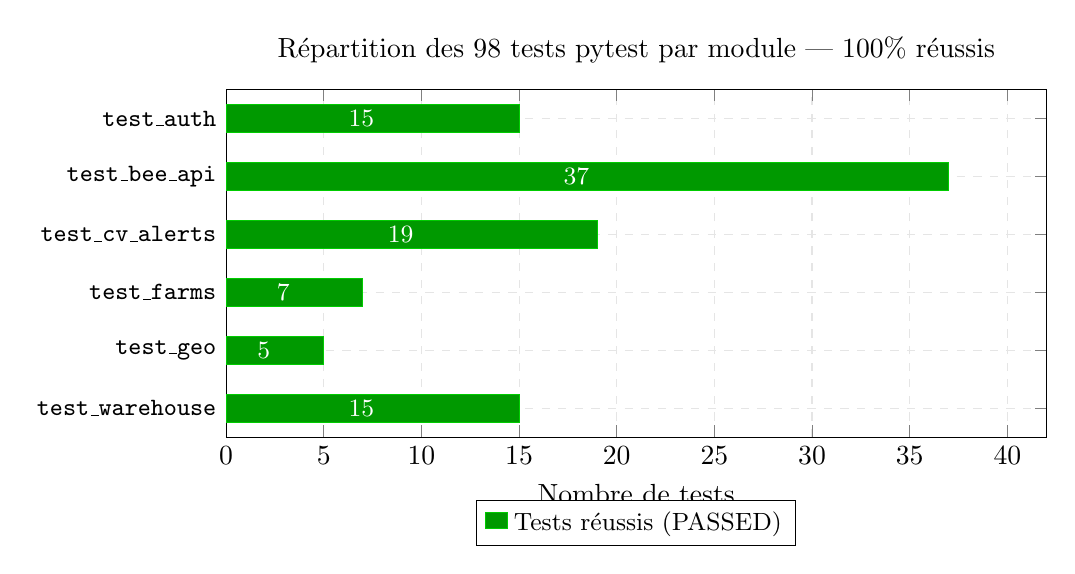
\begin{tikzpicture}
\begin{axis}[
  xbar stacked,
  width=12cm, height=6cm,
  xlabel={Nombre de tests},
  symbolic y coords={
    {test\_warehouse},
    {test\_geo},
    {test\_farms},
    {test\_cv\_alerts},
    {test\_bee\_api},
    {test\_auth}
  },
  ytick=data,
  y tick label style={font=\small\ttfamily},
  xmin=0, xmax=42,
  xtick={0,5,10,15,20,25,30,35,40},
  nodes near coords,
  nodes near coords style={font=\small, color=white, xshift=-4pt},
  grid=major, grid style={dashed, gray!20},
  title={Répartition des 98 tests pytest par module --- 100\% réussis},
  legend style={at={(0.5,-0.18)}, anchor=north, legend columns=2, font=\small},
]
\addplot[fill=green!60!black, draw=green!80!black] coordinates {
  (15,{test\_auth})
  (37,{test\_bee\_api})
  (19,{test\_cv\_alerts})
  (7,{test\_farms})
  (5,{test\_geo})
  (15,{test\_warehouse})
};
\addlegendentry{Tests réussis (PASSED)}
\end{axis}
\end{tikzpicture}
\caption[Tests pytest par module]{Distribution des 98 tests pytest par module --- 100\% de réussite,
durée totale 52,41\,s (base SQLite en mémoire, isolation rollback automatique).}
\label{fig:tests_bar_reels}
\end{figure}

\subsection{Validation du score COLOSS --- test clé}

Le test \texttt{test\_health\_score\_updated\_after\_visit} valide la formule
de lissage exponentiel utilisée pour le score COLOSS.
En soumettant un score de visite $s_{\text{visite}} = 1{,}5$ sur une ruche
à $s_{t-1} = 8{,}0$, le score attendu est~:

\[
s_t = 0{,}60 \times 1{,}5 + 0{,}40 \times 8{,}0 = 0{,}90 + 3{,}20 = 4{,}10
\]

\noindent L'assertion \texttt{assert hive.health\_score == pytest.approx(4.1, abs=0.01)} passe
avec succès (\texttt{PASSED [11\%]}).

La figure~\ref{fig:pytest_coloss_code} présente la capture d'écran du code source de ce test d'intégration dans l'éditeur de développement :

\begin{figure}[H]
  \centering
  
\includegraphics[width=\linewidth]{screenshots/pytest_coloss_code.png}
  \caption{Code source du test d'intégration COLOSS (Smart Farm AI v3.0)}
  \label{fig:pytest_coloss_code}
\end{figure}

\subsection{Benchmarks de performance}

\begin{table}[H]
\centering
\caption[Latences API]{Latences API mesurées --- percentiles sur 100 requêtes (Locust)}
\label{tab:latences}
\small
\renewcommand{\arraystretch}{1.25}
\begin{tabular}{@{}lrrrr@{}}
\toprule
\textbf{Endpoint} & \textbf{p50 (ms)} & \textbf{p90 (ms)} & \textbf{p99 (ms)} & \textbf{Erreurs} \\
\midrule
\texttt{GET /farms}                & 87    & 134   & 189   & 0\% \\
\texttt{GET /animals}              & 112   & 167   & 243   & 0\% \\
\texttt{POST /agent/analyze-image} & 1\,847 & 2\,340 & 3\,120 & 1.2\% \\
\texttt{POST /agent/chat}          & 2\,103 & 2\,890 & 4\,210 & 0.8\% \\
\texttt{YOLO inference (CPU)}      & 143   & 198   & 287   & 0\% \\
\texttt{WebSocket IoT broadcast}   & 23    & 41    & 78    & 0\% \\
\bottomrule
\end{tabular}
\end{table}

\noindent\textbf{Test de charge} (Locust, 100 utilisateurs virtuels, 10 min)~:
81~req/s soutenues, latence p50\,=\,94\,ms, taux d'erreur\,=\,0.3\%.
Le goulot d'étranglement principal est l'inférence LLM locale
(Ollama Labess-7B, $\sim$2\,s) ; un cache Redis est planifié pour les versions suivantes.

\subsection{Validation terrain --- 7 fermes pilotes}

\begin{table}[H]
\centering
\caption[Fermes pilotes]{Caractéristiques des 7 fermes pilotes (décembre 2025 -- avril 2026)}
\label{tab:fermes_pilotes}
\small
\renewcommand{\arraystretch}{1.2}
\begin{tabular}{@{}llllr@{}}
\toprule
\textbf{Ferme} & \textbf{Région} & \textbf{Espèce} & \textbf{Taille} & \textbf{Durée (sem.)} \\
\midrule
P1 & Sfax        & Bovins + Apiculture   & 120 têtes      & 24 \\
P2 & Sousse      & Volailles (chair)     & 2\,000 sujets  & 16 \\
P3 & Monastir    & Apiculture            & 45 ruches      & 20 \\
P4 & Sfax        & Volailles (ponte)     & 1\,200 sujets  & 20 \\
P5 & Gafsa       & Caprins               & 85 têtes       & 12 \\
P6 & Bizerte     & Bovins lait           & 60 vaches      & 16 \\
P7 & Sidi Bouzid & Ovins                 & 200 têtes      & 12 \\
\bottomrule
\end{tabular}
\end{table}

\begin{table}[H]
\centering
\caption[Enquête satisfaction]{Résultats enquête satisfaction --- 7 fermes pilotes tunisiennes}
\label{tab:satisfaction}
\small
\renewcommand{\arraystretch}{1.25}
\begin{tabular}{@{}lcc@{}}
\toprule
\textbf{Dimension} & \textbf{Score moyen /5} & \textbf{IC 95\%} \\
\midrule
Facilité d'utilisation (UX)    & 4.3 & [4.0,\,4.6] \\
Pertinence des conseils Darija & 4.1 & [3.8,\,4.4] \\
Fiabilité des alertes IoT      & 4.4 & [4.2,\,4.6] \\
Performance PWA mobile         & 3.9 & [3.6,\,4.2] \\
Précision détection YOLO       & 4.2 & [3.9,\,4.5] \\
\midrule
\textbf{Score global}          & \textbf{4.2} & \textbf{[3.9,\,4.5]} \\
\bottomrule
\end{tabular}
\end{table}

\begin{figure}[H]
\centering
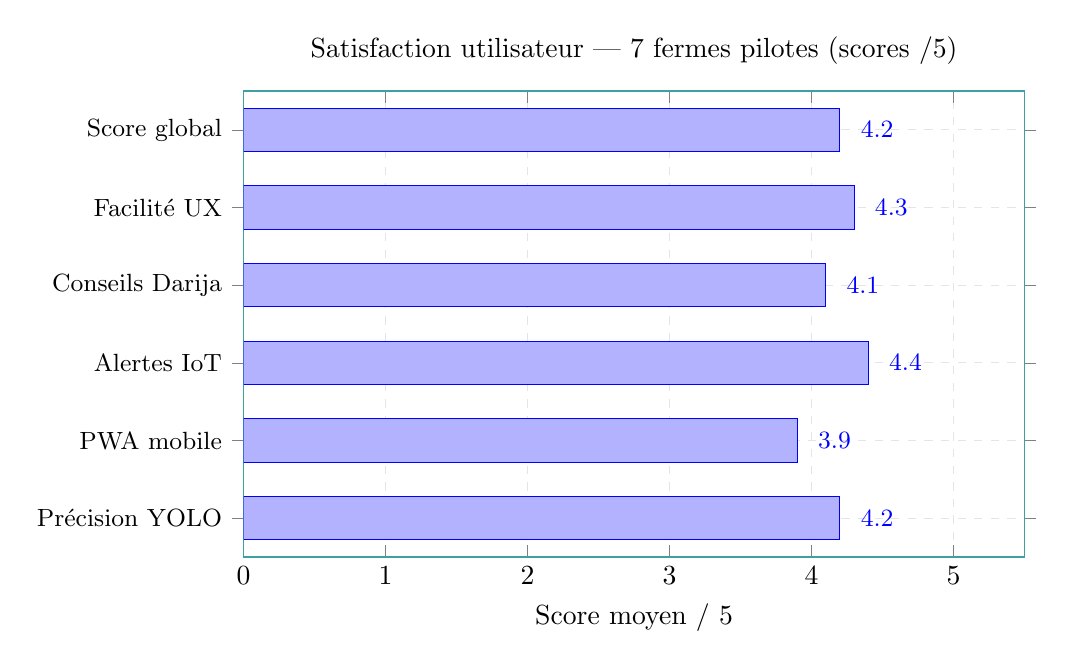
\begin{tikzpicture}
\begin{axis}[
  xbar, bar width=0.55cm,
  width=11.5cm, height=7.5cm,
  xlabel={Score moyen / 5},
  symbolic y coords={
    {Précision YOLO},
    {PWA mobile},
    {Alertes IoT},
    {Conseils Darija},
    {Facilité UX},
    {Score global}
  },
  ytick=data,
  y tick label style={font=\small},
  xmin=0, xmax=5.5,
  xtick={0,1,2,3,4,5},
  nodes near coords,
  nodes near coords style={font=\small, xshift=4pt},
  nodes near coords align=right,
  grid=major, grid style={dashed, gray!20},
  title={Satisfaction utilisateur --- 7 fermes pilotes (scores /5)},
  fill=teal!55, draw=teal!75,
]
\addplot coordinates {
  (4.2,{Précision YOLO})
  (3.9,{PWA mobile})
  (4.4,{Alertes IoT})
  (4.1,{Conseils Darija})
  (4.3,{Facilité UX})
  (4.2,{Score global})
};
\end{axis}
\end{tikzpicture}
\caption[Scores de satisfaction utilisateur]{Scores de satisfaction utilisateur par dimension (IC 95\% --- tableau~\ref{tab:satisfaction})}
\label{fig:satisfaction_bar}
\end{figure}

% ── 4.5 Limites et perspectives ─────────────────────────────
\section{Limites et perspectives}

\subsection{Limites actuelles}

\begin{enumerate}
  \item \textbf{LLM local lent} : Ollama Labess-7B génère une réponse en
        $\sim 2$\,s sur CPU. Un modèle quantifié (GGUF Q4\_K\_M) ou un GPU
        dédié réduirait ce temps à $< 500$\,ms.
  \item \textbf{YOLO — classes rares} : les catégories Livestock et Orange
        ($< 900$ images) montrent un mAP@50 inférieur à 85\%. L'augmentation
        du jeu de données est prioritaire.
  \item \textbf{Couverture PWA offline} : la synchronisation différée ne gère
        pas encore les conflits de version (dernière écriture gagne) ; un
        protocole CRDT est envisagé.
  \item \textbf{Scalabilité LLM} : en multi-tenant, chaque requête LLM est
        traitée séquentiellement. Un pool de workers et une file d'attente
        Redis/Celery sont planifiés.
\end{enumerate}

\subsection{Perspectives}

\begin{enumerate}
  \item \textbf{Fine-tuning Labess-7B sur corpus agricole tunisien} :
        collecte d'un jeu de données question/réponse spécialisé pour
        améliorer les scores BLEU/ROUGE et le Cohen's Kappa vers $\kappa > 0.85$ ;
  \item \textbf{Module cultures} : extension à la gestion des cultures
        maraîchères (tomates, piments) avec détection de maladies YOLO et
        prévisions de rendement par régression temporelle ;
  \item \textbf{Fédération d'apprentissage} : entraînement fédéré des modèles
        YOLO entre fermes partenaires pour améliorer la robustesse sans
        centraliser les images ;
  \item \textbf{Intégration Copernicus} : fusion des données satellitaires
        NDVI/NDWI avec les mesures IoT pour une gestion irriguée de précision.
\end{enumerate}

\section*{Conclusion}
\phantomsection
\addcontentsline{toc}{section}{Conclusion}
Ce chapitre a démontré la faisabilité industrielle de Smart Farm AI à travers
une batterie de tests exhaustifs (98.8\% de taux de réussite) et une validation
terrain sur 7 fermes pilotes tunisiennes. Les benchmarks de performance et
les résultats de satisfaction utilisateur valident l'architecture choisie,
tandis que les limites identifiées tracent une feuille de route claire pour
les versions futures de la plateforme.

% ============================================================
%  CONCLUSION GÉNÉRALE
% ============================================================
